%
% Modified version of the sample_ndthesis.tex
% by Sameer Vijay
% Last Change: Wed Jul 27 2005 14:00 CEST
%
%%%%%%%%%%%%%%%%%%%%%%%%%%%%%%%%%%%%%%%%%%%%%%%%%%%%%%%%%%%%%%%%%%%%%%%%
%
% Sample Notre Dame Thesis/Dissertation
% Using Donald Peterson's ndthesis classfile
%
% Written by Jeff Squyres and Don Peterson
%
% Provided by the Information Technology Committee of
%   the Graduate Student Union
%   http://www.gsu.nd.edu/
%
% Nothing in this document is serious except the format.  :-)
%
%%%%%%%%%%%%%%%%%%%%%%%%%%%%%%%%%%%%%%%%%%%%%%%%%%%%%%%%%%%%%%%%%%%%%%%%
% This is *not* a substitute for Donald's orginial documentation.  See
% /afs/nd.edu/usr/local/src/tex/texmf/doc/latex/ndthesis/ndthesis.dvi
% for documentation on the particular commands and whatnot.
%%%%%%%%%%%%%%%%%%%%%%%%%%%%%%%%%%%%%%%%%%%%%%%%%%%%%%%%%%%%%%%%%%%%%%%%
%
% You should *also* have a ND formatting guide to ensure that you have
% all the relevant parts, put the captions in the right place, etc.
% Just because you have this wonderful style classfile doesn't mean
% that it removes *all* the formatting onus from you.  :-)
%
% Normally, you should break all of this stuff up into separate files
% (at the very least, one chapter per file) and use the \input
% command.  This is all one file for brevity's (and clarity's) sake.
%
% Note that you should also have a good Makefile; one that invokes
% LaTeX as many times as necessary (up to 4) and bibtex if necessary.
% One should be included in this distribution.  You may want to modify
% the Makefile to make separate chapters, if necessary.
%
% If you have any suggestions, comments, questions, please send e-mail
% to: ndthesis@gsu.nd.edu
%
%%%%%%%%%%%%%%%%%%%%%%%%%%%%%%%%%%%%%%%%%%%%%%%%%%%%%%%%%%%%%%%%%%%%%%%%

\documentclass[textrefs,review]{nddiss2e}

% % uncomment the following line 
% if using chapter-wise bibliography
% \usepackage{chapterbib}
% \renewcommand{\bibname}{Cited Works}
% \renewcommand{\bibsection}{\section{\bibname}}

\begin{document}

\frontmatter

\title{Potential of Opportunistic Relaying\\ {\small\scshape Performance study across wireless interfaces on smartphones} }
\author{Shu Liu}
\work{Dissertation}
\degprior{B.S., M.S.}
\degaward{Doctor of Philosophy\\in\\Computer Science and Engineering}
\advisor{Aaron Striegel}
% \secondadvisor{Gordon Gray}
\department{Computer Science and Engineering}

\maketitle
%%%%%%%%%%%%%%%%%%%%%%%%%%%%%%%%%%%%%%%%%%%%%%%%%%%%%%%%%%%%%%%%%%%%%%%%
%
% Front stuff
%
%%%%%%%%%%%%%%%%%%%%%%%%%%%%%%%%%%%%%%%%%%%%%%%%%%%%%%%%%%%%%%%%%%%%%%%%

\copyrightholder{Shu Liu}
\copyrightyear{2014}
\makecopyright

\begin{abstract}
\end{abstract}

\renewcommand{\dedicationname}{}

\begin{dedication}
  To my husband, Wei, who inspires me to exceed my potential. 
\end{dedication}

\tableofcontents
\listoffigures
\listoftables

\begin{preface}
\end{preface}

\begin{acknowledge}
I would like to thank my advisor, Dr. Aaron Striegel, who helped provide
direction and guidance for this work. Without his trust and support, I would not have had the opportunity to work in such great research projects. I would also like to thank the members of my committee, Dr. Christian Poellabauer, Dr. David Hachen and Dr. Gregory Madey, for their time and support in this process.

I also need to thank all my colleagues who create such a good atmosphere in the group;
Dr. Andrew Blaich, Dr. Yingxin Jiang, Dirk Van Bruggen, Lei Meng, Xueheng Hu, Benjamin Bockdtege, and Rachael Purta.  Also Margaret and Michael, deserve a special thanks because their great supports in the Netsense project. I need to further thank all my friends, Nikhil, Hongsheng and Mehrdad, who always took the time to listen. 
\end{acknowledge}

\begin{symbols} 
\end{symbols}

\mainmatter

%
% Chapter 0 (features)
%
\setcounter{chapter}{-1}
\chapter{FEATURES OF FORMATTING IN THIS EXAMPLE FILE}

This \verb+chapter+ has been added to the original sample file to highlight the
various features with the formatting that conforms to the Graduate school
guidelines --- whether obtained due to the use of \nddiss\/ class file or just
plain good practice.
\begin{itemize}
\item An important thing you might notice is that the title of this chapter 
is not in all CAPS. This is a feature since using \verb+\MakeTextUpperCase{}+ 
is not helpful
when you have a math formula or something that just doesnt go CAPS (for eg.
elemental symbols).
\item If you're looking at a pdf document, the pdf bookmarks (left column) link
to all major textual sections including abstract, toc, lof, lot and
bibliography.
\item In the {\em dedication}, the title name has been modified. So, you know
how to and that it can be done.
\item The entries in the {\em List of figures} and {\em List of Tables} are
single-spaced themselves but are double-spaced from the other.
\item The table captions are not in all CAPS as well for the reason mentioned
above.
\item Appropriate space is left between the \verb+Table xx+ and its
corresponding caption (which is double-spaced itself) as in table \ref{tbl:bogus1}.
\item Tables look much better without the vertical lines (good practice).
\item There is double-spacing between the table entries but single-spacing
within the entry.
\item The chapter (see Chapter \ref{chap:golfing}) or section titles are
double-spaced as mentioned in the guidelines.
\item There is a \verb+subsubsection+ present (eg. section \ref{sec:data}) and
is properly formatted in the TOC.
\item Table \ref{tbl:defs} is an example of the use of \textsf{landscape}
environment in which a normal table is formatted in a {\em landscape} mode.
\item The \textsf{longtable} environment is used in Tables \ref{tbl:votes} and
\ref{tbl:rotated-rankings}, in normal and \verb+landscape+ mode, respectively. The
table captions are formatted properly in both cases.
\item In the table \ref{tbl:votes}, the \verb+footnote+ in the table header 
does not appear at all. This is not an error of the \nddiss\/ class but of the
\textsf{longtable} package.
\item An example of citing a website is shown in the bibliography (see
\citep{gairley2000}) which is formatted using the 
\verb+nddiss2e.bst+
citation style file.
\item A bit of information on the \nddiss\/ class file and the typesetting program
used is included in a box on the last page of the thesis.
\end{itemize}

%
% Chapter 1
%

%
% Modified by Sameer Vijay
% Last Change: Tue Jul 26 2005 13:00 CEST
%
%%%%%%%%%%%%%%%%%%%%%%%%%%%%%%%%%%%%%%%%%%%%%%%%%%%%%%%%%%%%%%%%%%%%%%%%
%
% Sample Notre Dame Thesis/Dissertation
% Using Donald Peterson's ndthesis classfile
%
% Written by Jeff Squyres and Don Peterson
%
% Provided by the Information Technology Committee of
%   the Graduate Student Union
%   http://www.gsu.nd.edu/
%
% Nothing in this document is serious except the format.  :-)
%
% If you have any suggestions, comments, questions, please send e-mail
% to: ndthesis@gsu.nd.edu
%
%%%%%%%%%%%%%%%%%%%%%%%%%%%%%%%%%%%%%%%%%%%%%%%%%%%%%%%%%%%%%%%%%%%%%%%%


%
% Chapter 1
%

\chapter{INTRODUCTION}

\section{Overview}

Over the past few years, a vast array of wireless devices and services have emerged that are fundamentally transforming how we as a society gather and react to information.  Furthermore, the new wireless ecosystem has increased wireless data consumption at phenomenal rates with the most popular cited estimates slating traffic to double every year for the next five years \cite{CiscoAnnualCellGrowth}.  Dubbed the \emph{wireless data tsunami}, the dominant question for wireless service providers (carriers) is how to meet what appears to be an insatiable need for wireless data.  Unlike wired networks, spectrum available for wireless data is finite and typically entails massive costs for acquisition and infrastructure deployment.  Although
technologies such as LTE herald the arrival of fourth-generation (4G) wireless technology, the new speeds often only temporarily satiate the need for additional bandwidth. A wide variety of solutions have emerged ranging simpler solutions such as better WiFi offloading to much more complex solutions such as small heterogeneous cellular networks. For many cellular providers, WiFi offloading, i.e. the users receiving data from 802.11-based hotspots, offers a significant appeal by reducing the strain on the already overloaded cellular infrastructure. Recent studies such as the one in \cite{lee2010mobile} points to offloading offering gains approaching 65\% of the total traffic volume. There are other works such as \cite{balasubramanian2010augmenting, dimatteo2011cellular, han2011mobile, icc2012performance} that discuss the feasibility of WiFi offloading. 

Besides WiFi offloading, a rich category of work that is complementary to existing techniques is the concept of \emph{opportunistic communication}. Opportunistic communication refers to the concept which allows nodes to leverage sporadic, intermittent contacts when two nodes come into direct radio communication range~\cite{pelusi2006opportunistic}. When cellular or WiFi links are not available or not strong enough, opportunistic relaying introduces another alternative option for mobile device to get connected by working in tandem with one or more devices.  From a conceptual standpoint for opportunistic networking, the design of the relaying protocol is critical, namely how does one select and manage appropriate relaying nodes as relays~\cite{laneman2004cooperative,sendonaris2003user,bletsas2006simple,lu2009design,bahl2009opportunistic}.  From a practical standpoint for opportunistic networking, it is essential to prove the potential for opportunistic relaying amongst actual mobile device users in real world. 

The primary goal of my work is to gather high quality smartphone data and leverage the data for reinforcing analysis from a technical network system perspective with respect to network connectivity and performance enhancement. In particular, I answered three interrelated questions: \emph{(i) Can existing wireless technologies on smartphone provide accurate face-to-face proximity estimation and to what extent are relationship formation and maintenance dynamics modified with the introduction of digital communication? (ii) Can the WiFi offloading be the ultimate solution for the predicted wireless data tsunami? (iii) Can the peer-to-peer communication between mobile devices in close proximity be a good candidate for offloading cellular systems?} The answers to these questions are fascinating to explore. The NetSense project is a study of first-year students tracked over a two-year period with respect to nearly all the smartphone information. The process of gathering data results in a rich pool of digital data which provides us the opportunities to analyze the technical dynamics of the network. These involve for instance, the wireless signal strengths can reflect the relative distance and connection status. Moreover, by collecting the information of traffic consumed by the phones, we are able to compare different types of traffic usage and understand their impacts on campus wireless networks. 

\section{Contributions}
The key contributions of my dissertation is as follows:
\begin{itemize}
\item Smartphone monitoring system: By collecting data on Android smartphones, we get a fully anonymized dataset containing device information and digital communication data of participants. It is the foundation of the research and provides multiple dimensions of data for research in both network science and sociology. 

\item Bluetooth proximity: Under the premise that Bluetooth has better accuracy for short distance without the constrain of environment, we use Bluetooth signal strength as an indicator for relative distance between devices. In order to get accurate estimation of face-to-face distance, a proximity estimation model is proposed by leveraging the raw Bluetooth Received Signal Strength Indicator (RSSI) values and introducing multiple thresholds for different environments. 

\item WiFi offloading: For most cellular providers, WiFi offloading appeals to reduce the strain on the overloaded cellular infrastructure. However, based on our data, the WiFi traffic takes approximately 30\% of the total data consumption which is much lower than expected. We analyze the possible reasons for this as well as the usage patterns of users in different categorization according to their WiFi traffic consumption. 

\item Proximity relay: 
With the support of peer-to-peer communication in smartphones, it is practical to leverage the device-to-device data transfers to bridge the coverage gap between cellular and WiFi infrastructure network. Based on our data, we will do the quantitative analysis of the potential relaying which is a key missing part in relaying related research and evaluate the benefits of relaying for cellular traffic offloading in real life. 
\end{itemize}

The rest of this paper is organized as follows. Section~\ref{sec:related_work} provides an overview of the related work and Section~\ref{sec:dataset} introduces the dataset we have. Based on the dataset, the framework to evaluate the potential for relaying is proposed in Section~\ref{sec:potential}. In the end, Section~\ref{sec:conclusion} concludes the paper.



%
% Chapter 2
%

%
% Modified by Sameer Vijay
% Last Change: Wed Jul 27 2005 13:00 CEST
%
%%%%%%%%%%%%%%%%%%%%%%%%%%%%%%%%%%%%%%%%%%%%%%%%%%%%%%%%%%%%%%%%%%%%%%%%
%
% Sample Notre Dame Thesis/Dissertation
% Using Donald Peterson's ndthesis classfile
%
% Written by Jeff Squyres and Don Peterson
%
% Provided by the Information Technology Committee of
%   the Graduate Student Union
%   http://www.gsu.nd.edu/
%
% Nothing in this document is serious except the format.  :-)
%
% If you have any suggestions, comments, questions, please send e-mail
% to: ndthesis@gsu.nd.edu
%
%%%%%%%%%%%%%%%%%%%%%%%%%%%%%%%%%%%%%%%%%%%%%%%%%%%%%%%%%%%%%%%%%%%%%%%%

%
% Chapter 2
%

\chapter{Large-scale Dataset}
\label{chap:dataset}
As espoused by the MIT Reality Mining group in \cite{Nathan3,Nathan1}, the increasing availability and reliability of smartphones affords incredible opportunities for the unobtrusive gathering of data with regards to usage, location, and performance.  Although quite expensive to gather versus user self-reporting or user volunteers, a fully instrumented smartphone represents a veritable wealth of data that can afford unique insight into the smartphone performance study.

In August of 2011, two hundred participants were selected from the incoming freshmen class of our university and received a free Android smartphone and plan in exchange for agreement to participate in the two-year data collection project.  Each Android device was rooted and a custom ROM installed (Cyanogenmod) to enable the device being permanently Bluetooth discoverable. A user-level agent was installed on each of the smartphones that extracted a wide variety of environmental and usage data from the phone at periodic intervals.  The monitoring agent was installed to start automatically when the smart phone power was turned on and ran passively in the background. Tuning was conducted on the agent to ensure that even with WiFi enabled and Bluetooth always discoverable for a battery life potential at distribution of roughly one and a half days.  

\section{Data Collection}
In order to build a flexible and stable platform for delivering on-going subject queries in a secure and efficient way, we designed and implemented the monitoring system in the Fall of 2010 and did a few serials of tests before the study began. The key part of the monitoring system is the customized agent installed on the smartphones named \textit{PhoneMonitor} as illustrated in Figure~\ref{fig:agent}. The Android platform was selected for its customization capabilities through normal API or rooted/customized interfaces with respect to hardware-level interactions. It collects a variety of types of data as illustrated in table~\ref{table:data} and each kind of data is invoked through the corresponding function calls. Separate threads are employed to compensate for the variety of speeds at which the respective functions retrieve relevant data. For example, the Bluetooth data includes the detailed values of timestamp, RSSI (Received signal strength indication), MAC address, and Bluetooth identifier (BTID) with a default sensing granularity of once per minutes. The wireless environmental data (primarily WiFi) has similar fields except the access point (AP) name is recorded and the granularity of sensing is three minutes. Traffic data includes breakdowns by application and wireless adapter (cell, WiFi) with respect to both downlink (Rx) and uplink (Tx) usage at intervals down to as low as once per minute. The light sensor data, which includes the timestamp and sensor values, can help us to determine whether the phone is sheltered (e.g. inside a backpack or in hand) and the surroundings (e.g. inside or outside buildings) during the daytime. It is recorded if the current value changes more than 30 compared with the last recorded value. For mail data, both sender and receiver email addresses are recorded without content snooping. More detailed information about collected data can be found in table~\ref{table:detailed_data}. Graphic User Interface (GUI) of the application allows participants to read the last check-in time as well as the status of the network connection and Bluetooth. 

\begin{figure}[h!tbp]
\centering 
{\includegraphics[width=3.5in]{graphs/Figure1.eps}}
\caption{Design of PhoneMonitor} 
\label{fig:agent}
\end{figure} 

\begin{table}[ht] 
\caption{Types of data collected in PhoneMonitor application} 
\centering  
\begin{tabular}{|l|m{10cm}|}
\hline
{\bf Device Information} & Bluetooth, WiFi, Cell, Location, Light Sensor, Screen On/Off, Battery Level, Connection Status, Network Traffic, Application Usage, Port Information, Running/Install Apps, Password, Contacts, Camera Usage\\
\hline
{\bf Digital Communication} & Phone Call, SMS, Mail, Web Browser History, Music\\
\hline
\end{tabular}
\label{table:data} 
\end{table}

Figure~\ref{fig:system} illustrates the framework of smartphone data collection, storage and query process. Data is locally spooled on the phone before being securely transmitted to one of two remote check-in servers.  Data from the check-in server is then spooled locally before being conveyed to a database server not directly connected to the Internet with all accesses strictly logged and validated to protect sensitive user data. From September 2011 to September 2013, we got more than 250G data in the database. 

\begin{figure}[h!tbp]
\centering 
{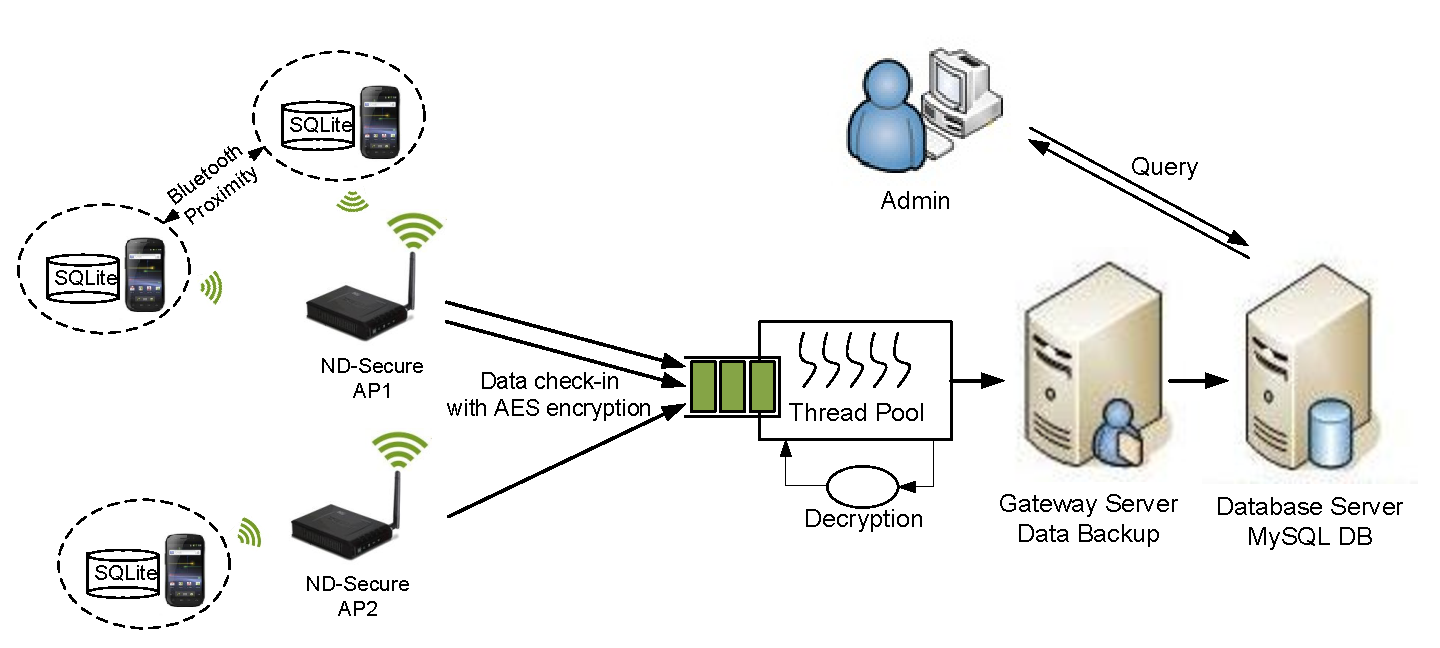
\includegraphics[width=6in]{graphs/system.eps}}
\caption{Smartphone monitoring system} 
\label{fig:system}
\end{figure} 

\section{Dataset Overview}
The dataset used in the dissertation covers 15 months data (Oct 2011 - Dec 2012) and there are around 41 million Bluetooth records, 50 million WiFi scans and 1 million SMS messages. Data from the first two months of the study is excluded to allow for the new freshmen to have settled into a new routine and social arrangements.  A reasonable degree of co-location exists amongst students in the study with students selected clustered amongst six primary dormitories equally divided amongst male and female students.  Once entered into the study, students were free to re-locate at either the beginning of the spring semester (2012) or the start of their sophomore year.  Moreover, the respective distribution levels within individual dormitories made it reasonably close to random chance amongst incoming freshmen for that dormitory if two participants in the study were selected as roommates. At the onset of the monitored period for the paper, approximately 11 students had dropped from the student reducing the data pool to 189 students.  

Table~\ref{table:summary} summarizes the details of the data across different months.  For each of the respective metrics presented in the table, we reduce the sampling rate to five minutes slots scattered throughout the day where each day has the potential for 288 measurement points.  The powered on percentage represents the number of slots when the phone monitor was active with a noticeable drop during later hours (12am - 8 am) but a notable uptick during the evening hours (4pm-12am).  The screen on percentage is the duration when the phone screen is on and implies the average usage of the phone for either consuming data or conducting other communications (SMS, phone call, etc.).  The monthly Bluetooth and WiFi records shows the average number of distinguished Bluetooth devices/WiFi APs detected per device across the month.  University virtual APs are reduced to a single AP as each university router offers between two to four WiFi AP names.  

Figure~\ref{fig:num_cdf} exhibits the empirical distribution functions (ECDF) of different types of data in April 2012 to offer additional context for the data beyond the average values denoted in Table \ref{table:summary}.  Two percentage value ECDFs are plotted (power on, screen on) together with two detected environmental values (unique Bluetooth devices in the month, unique APs in the month).  Scales for each of the two values are the lower axis for percentage and upper axis for raw numeric counts.   Most notably, the average number of unique Bluetooth devices detected in April 2012 was 746 with some devices seeing as high as over 1000 devices and others seeing as low as slightly less than 200 unique devices.  Table~\ref{table:summary} also contains distinctions with respect to intra-study proximity and inter-study breakdowns of the various Bluetooth devices.  As would be expected, intra-study detection dramatically trails off during summer break in tandem with detected university APs as the students leave campus.       

\begin{table}[tb] 
\caption{Monthly Data Summary} 
\centering
\begin{tabular}{p{6cm}|c|c|c|c}
\hline
		  Avg. Monthly Values per Phone							& Nov 2011 & Apr 2012 & Jul 2012 & Nov 2012 \\ [0.5ex] 
\hline\hline Powered On (\%) 										& 73.7 	   & 70.6 	      & 51.3 	& 61.2		\\ 
\hline	  Powered On (\%) (12am-8am) 							&  66.7	    & 60.7 		& 42.3 	& 58.0 \\
\hline 	  Powered On (\%) (8am-4pm) 								& 74.6 	   & 69.3 	      & 51.3 	& 62.7 \\
\hline 	  Powered On (\%) (4pm-12am)   			 				& 79.6	    & 72.7 		& 60.1 	& 62.9 \\
\hline	  Screen On (\%)										&  5.74	    & 5.05 		& 4.99 	& 4.30 \\
\hline	  Total Rx Traffic  (MB)									&  609.2	    & 727.2 	& 864.5 	& 685.8 \\
\hline	  Total Tx Traffic  (MB)									&  133.11	    & 123.8 	& 130.4 	& 200.8 \\
\hline 	  \# of Detected Distinct Bluetooth Devices					&  961 	     & 746 		& 310 	& 681	 \\
\hline 	  \# of Detected Distinct Bluetooth Devices Within Project (RSSI $>=$ -80dBm) 	&  131 	     & 106 		 & 	$<$1 & 75	 \\
\hline	  \# of Detected Distinct WiFi APs 										&  1218 	     & 1004	 	& 1777 	& 1663 \\
\hline	  \# of Detected Distinct WiFi APs in Campus 								&  424 	     & 446	 	& $<$1 	& 433 \\
\hline
\end{tabular}
\label{table:summary} 
\end{table}

\begin{figure}[tbp]
\centering 
{\includegraphics[width=3.5in]{graphs/num_cdf.pdf}}
\caption{ECDF of Data in April 2012} 
\label{fig:num_cdf}
\end{figure} 

\section{Comparison}
The inclusion of a device-side agent on a live user device introduces notable complexity with respect to user privacy and IRB (Institutional Review Board) concerns.  Moreover, such studies tend to be frequently expensive to conduct due to the cost of subsidizing access costs at a sufficient level to yield effective participatory compliance. Although there are several notable wireless datasets including university campuses (MIT Reality~\cite{Nathan3}, UCSD~\cite{mcnett2005access} and Dartmouth~\cite{henderson2004changing}), conference sites (Infocom~\cite{chaintreau2007impact}) and cities (Nokia~\cite{laurila2012mobile}), most datasets are limited in size and scope in terms of capturing dyadic relationships, namely both sides of a potential proximity relationship for the purposes of truly evaluating opportunistic networking.  For instance, both the MIT Reality and Infocom traces record when contact is detected by virtue of Bluetooth discovery, ample for characterizing the inter-contact times but not necessarily capturing energy levels nor traffic needs of the respective nodes.  Alternatively, the UCSD and Dartmouth traces rely on WiFi for localization gathering either data via AP fingerprinting (UCSD) or SNMP logs directly from the AP (Dartmouth).  The richest of the datasets is the data from the Nokia Data Challenge which includes both WiFi and Bluetooth data but the dataset is no longer public after the completion of the analysis.  In contrast to prior works, our dataset includes nominal proximity (Bluetooth) / location data (WiFi, Google Location service) in addition to a complete view of the smartphone environment including WiFi signal strengths, energy levels, traffic demands, and the social context for the participants in the study (Facebook, SMS, etc.).  Table~\ref{table:datasets} summarizes the most relevant studies and compares the works to our own reference study.  

\begin{landscape}
\begin{table*}[t] 
\caption{Dataset Comparison} 
\centering
\scalebox{1}{
\begin{tabular}{c|c|c|c|c|c|c}
\hline
  			Traces 				&  Our Dataset  	&  MIT Reality 	 & 	UCSD 		& Dartmouth 	& Infocom  	& Nokia \\ [0.5ex] 
\hline
\hline		Device  				& Smartphone		&  Cell Phone	 & 	PDA			& Laptop PDA & iMote		&Smartphone \\
\hline		\# of Devices 			& 189			& 97			 & 	275			& 6,648		& 41			& 185\\
\hline		Network Type 			&  Bluetooth/WiFi	& Bluetooth	 &     WiFi			& WiFi 		& Bluetooth	& Bluetooth/WiFi\\
\hline		Contact Type 			& Direct/AP-based	& Direct		 & 	AP-based		& AP-based	& Direct		& Direct/AP-based\\
\hline		Duration (days)			& 458			& 246		 & 	77			& 114		& 4			& 210\\
\hline		Granularity (seconds) 	& 60/300			& 300		 & 	120			& 300		& 120		& N/A\\
\hline		\# of internal contacts 	& 3,616,184 		& 54,667		 &	195,364		& 4,058,284	& 22,459		& N/A\\
\hline		Internal pairwise contact/day	& 0.221		& 0.022		 & 	 0.034		& 0.008		& 3.4		& N/A\\	
\hline		Other proximity related data	& Cell, Traffic, etc.	& Cell	 & 	N/A			& N/A		& N/A		& Cell, etc.\\
\hline
\end{tabular}}
\label{table:datasets} 
\end{table*}
\end{landscape}



%
% Appendix
%

\appendix

%
% Modified by Sameer Vijay
% Last Change: Wed Jul 27 2005 13:00 CEST
%
%%%%%%%%%%%%%%%%%%%%%%%%%%%%%%%%%%%%%%%%%%%%%%%%%%%%%%%%%%%%%%%%%%%%%%%%
%
% Sample Notre Dame Thesis/Dissertation
% Using Donald Peterson's ndthesis classfile
%
% Written by Jeff Squyres and Don Peterson
%
% Provided by the Information Technology Committee of
%   the Graduate Student Union
%   http://www.gsu.nd.edu/
%
% Nothing in this document is serious except the format.  :-)
%
% If you have any suggestions, comments, questions, please send e-mail
% to: ndthesis@gsu.nd.edu
%
%%%%%%%%%%%%%%%%%%%%%%%%%%%%%%%%%%%%%%%%%%%%%%%%%%%%%%%%%%%%%%%%%%%%%%%%

%%%%%%%%%%%%%%%%%%%%%%%%%%%%%%%%%%%%%%%%%%%%%%%%%%%%%%%%%%%%%%%%%%%%%%%%
%
% Appendix
%
%%%%%%%%%%%%%%%%%%%%%%%%%%%%%%%%%%%%%%%%%%%%%%%%%%%%%%%%%%%%%%%%%%%%%%%%

\begin{table}[ht] 
\caption{Detailed Information of Collected Data } 
\centering  
\begin{tabular}{c|l|l}
\hline
		  Type			& Collected Information 					& Frequency \\ [0.5ex] 
\hline\hline Location			& Provider/Latitude/Longitude/Accuracy		& 10 min/100 meters	\\ 
\hline	  Bluetooth 		& ID/MAC/RSSI	    						& 1 min \\
\hline 	  WiFi 			& AP name/MAC/RSSI					& 3 min \\
\hline 	  Cell   			& 									& when RSSI changes \\
\hline	  Battery			& Charge method/Level	    				& when level changes at least 1 \\
\hline	  Light			& Level	    							& when level changes at least 30 \\
\hline	  Screen			& On/Off 							 	& when screen on/off \\
\hline 	  Camera			& Picture/Video name			        	        & when created	 \\
\hline 	  Network Traffic 	& Type/Cumulative bytes					& 1 min	 \\
\hline	  App Traffic		& Type/Name/Cumulative bytes			& 1 min \\
\hline	  App Status 		& Name/Permission/Total number			& 1 day \\
\hline 	  Port Traffic	        & Protocal/State/Pid/Src/Dst/Name			& 15 min \\
\hline 	  Password	  	& Type/Encrypted pwd/Salt				& 1 hour \\
\hline 	  Contacts			& Phone number/Email/Total number		& 1 day \\
\hline 	  Connection		& Status								& when status changes \\
\hline 	  Storage			& Total vol/Free vol						& 12 hours \\
\hline 	  Version			& Version number							& when phone starts \\
\hline 	  Phone Call		& Number/Duration						& 1 hour \\
\hline 	  SMS			& Number/Length						& 1 hour \\
\hline 	  MMS			& Number/Type						& 1 hour \\
\hline 	  Mail			& Sender/Receiver/						& 6 min \\
\hline 	  Music			& Album name/Display name/Size			& 3 min \\
\hline 	  Browser History	& Title/Url/Visited Times					& 1 hour \\
\hline
\end{tabular}
\label{table:detailed_data} 
\end{table}



%
% Back stuff
%

% % comment out the following three lines
% if using chapter-wise bibliography

 \backmatter
 \bibliographystyle{nddiss2e}
 \bibliography{dissertation}

\end{document}

% End of ``example.tex''
